%%%%%%%%%%%%%%%%%%%%%%%%%%%%%%%%%%%%%%%%%
% University Assignment Title Page 
% LaTeX Template
% Version 1.0 (27/12/12)
%
% This template has been downloaded from:
% http://www.LaTeXTemplates.com
%
% Original author:
% WikiBooks (http://en.wikibooks.org/wiki/LaTeX/Title_Creation)
%
% License:
% CC BY-NC-SA 3.0 (http://creativecommons.org/licenses/by-nc-sa/3.0/)
% 
% Instructions for using this template:
% This title page is capable of being compiled as is. This is not useful for 
% including it in another document. To do this, you have two options: 
%
% 1) Copy/paste everything between \begin{document} and \end{document} 
% starting at \begin{titlepage} and paste this into another LaTeX file where you 
% want your title page.
% OR
% 2) Remove everything outside the \begin{titlepage} and \end{titlepage} and 
% move this file to the same directory as the LaTeX file you wish to add it to. 
% Then add \input{./title_page_1.tex} to your LaTeX file where you want your
% title page.
%
%%%%%%%%%%%%%%%%%%%%%%%%%%%%%%%%%%%%%%%%%

%----------------------------------------------------------------------------------------
%	PACKAGES AND OTHER DOCUMENT CONFIGURATIONS
%----------------------------------------------------------------------------------------

\documentclass[12pt,spanish]{article}
\usepackage[spanish]{babel}
\selectlanguage{spanish}
\usepackage[utf8]{inputenc}
\usepackage{makeidx}
\usepackage{graphicx}
\usepackage{hyperref}
\begin{document}

\begin{titlepage}

\newcommand{\HRule}{\rule{\linewidth}{0.5mm}} % Defines a new command for the horizontal lines, change thickness here

\center % Center everything on the page
 
%----------------------------------------------------------------------------------------
%	HEADING SECTIONS
%----------------------------------------------------------------------------------------

\textsc{\LARGE Práctica 1.b}\\[1.0cm] % Name of your university/college
\textsc{\Large Búsqueda por Trayectorias}\\[0.5cm] % Major heading such as course name
\textsc{\large Selección de características}\\[0.5cm] % Minor heading such as course title

%----------------------------------------------------------------------------------------
%	TITLE SECTION
%----------------------------------------------------------------------------------------

\HRule \\[0.4cm]
{Algoritmos considerados: SFS,LS,SA,BT básico}\\[0.4cm] % Title of your document

 
%----------------------------------------------------------------------------------------
%	AUTHOR SECTION
%----------------------------------------------------------------------------------------

\begin{minipage}{1\textwidth}
\begin{flushleft} \large
Luis Suárez Lloréns\\
DNI: 75570369-M\\
luissuarez@correo.ugr.es\\
5º Doble Grado Ingeniería Informática y Matemáticas\\
Grupo de Prácticas: 3
\end{flushleft}
\end{minipage}

% If you don't want a supervisor, uncomment the two lines below and remove the section above
%\Large \emph{Author:}\\
%John \textsc{Smith}\\[3cm] % Your name

%----------------------------------------------------------------------------------------
%	DATE SECTION
%----------------------------------------------------------------------------------------

%----------------------------------------------------------------------------------------
%	LOGO SECTION
%----------------------------------------------------------------------------------------

%\includegraphics{Logo}\\[1cm] % Include a department/university logo - this will require the graphicx package
 
%----------------------------------------------------------------------------------------

\vfill % Fill the rest of the page with whitespace

\end{titlepage}
\tableofcontents
\newpage
\section{Descripción del problema}
Cuando se trata un problema de clasificación o de aprendizaje automático, nunca sabemos a priori los datos que nos serán útiles. Es más, añadir datos innecesarios puede incluso empeorar el rendimiento de nuestro clasificador.\\
 
 El fin del problema de selección de características es tratar de tomar un conjunto de datos de calidad, que nos permita afrontar el posterior aprendizaje de una manera más rápida y con menos ruido en los datos.\\
 
Pese a no ser este un problema directamente de clasificación, vamos a necesitarla para valorar la calidad de una solución del problema. Por tanto, necesitamos un clasificador sencillo para esta tarea. Utilizaremos el clasificador k-nn --- para ser más concreto, 3-nn ---, y trataremos de encontrar las características con las que mejor clasifique un conjunto de prueba.\\

Entonces, usando el clasificador 3-nn, nuestro objetivo va a ser maximizar la función:\\
 
 \[
 \	\frac{Instancias\, bien\, clasificadas}{Total\, de\, instancias}
 \]
 
 
\newpage
\section{Consideraciones generales}
En esta sección veremos los componentes en común de los diferentes algoritmos.
\begin{itemize}
\item Representación: Array binario con la misma longitud que el número de datos.
\item Función objetivo: Porcentaje de acierto del clasificador 3-nn. Para evaluarlo Tendríamos que hacer lo siguiente:
\begin{itemize}
\item Tomar las columnas que nos indique la solución.
\item Entrenar el clasificador con los datos de entrenamiento y sus etiquetas.
\item Clasificar los datos de test y comprobar si coinciden con sus verdaderas etiquetas.
\end{itemize} 
Además, para poder ver lo bien que clasifica al propio conjunto de entrenamiento, realizamos "Leave One Out", que consiste en, para cada dato del conjunto de entrenamiento, quitarlo de los datos de entrenamiento, clasificarlo y ver si hemos acertado al clasificar o no.
\item Generación de vecindario: El vecindario serán las soluciones que solo difieran de la actual un bit. La generación del vecino i-ésimo podría realizarse de la siguiente forma: Si el valor en la posición i es 1, ponerlo a 0.Si no, ponerlo a 1. 
\item Uno de los parámetros de los algoritmos a la hora de ejecutarlos es la solución inicial. Esto nos permitirá utilizar estos mismos métodos para la realización de búsqueda multiarranque, por ejemplo. Por tanto, el calculo de una solución de inicio aleatoria se encuentra fuera de los algoritmos.
\end{itemize}
\newpage
\section{Explicación de los algoritmos}

\subsection{BL}
Para generar de manera aleatoria los vecinos de una solución dada, realizamos lo siguiente:
\begin{itemize}
\item Crear una lista de números de 0 al número de características del problema
\item Reordenar aleatoriamente dicha lista
\end{itemize} 
La lista reordenada después se recorre, y modificando el elemento indicado de la solución de partida, obtenemos los vecinos.\\
Búsqueda local:
\begin{itemize}
\item Hasta que no encontremos mejora en el bucle interno o superemos el número máximo de iteraciones, repetir:
\item Para cada vecino, ordenados aleatoriamente ---bucle interno---
\begin{itemize}
\item Calcular la función objetivo.
\item Si mejora la función objetivo de la solución actual, pasa a ser la solución actual y termina el búcle interno.
\end{itemize} 
\end{itemize} 
\newpage
\subsection{ES}
Temperatura inicial:
\begin{itemize}
\item Calculamos la función objetivo de la solución inicial
\item Realizamos la operación $\frac{\mu * puntuacion}{-log(\phi)}$
\end{itemize}
Enfriamiento:
\begin{itemize}
\item Al inicio del programa, calculamos $\beta$ con la fórmula dada.
\item Para enfriar, realizamos $t_{k+1} = \frac{t_{k}}{1+\beta t_{k}}$
\end{itemize}
Enfriamiento simulado:
\begin{itemize}
\item Hasta que no encontremos mejora en el bucle interno, superemos el número máximo de iteraciones o la temperatura sea menor que la temperatura final, repetir:
\item Poner a 0 el número de soluciones aceptadas en este enfriamiento y hacer el número máximo de iteraciones en el bucle interno lo siguiente:
\begin{itemize}
\item Si has aceptado las suficientes, termina el bucle
\item Si no, toma un vecino aleatorio y calcula su función objetivo
\item Si es el mejor hasta ahora, tomalo como mejor solución y como siguiente solución y aumenta en uno el número de soluciones aceptadas.
\item Si no es el mejor, y tiene el mismo valor que el actual, pasamos al siguiente vecino ---Se hace así para evitar ciclos infinitos que nos impedían salir por la condición "no encontramos mejora---
\item Si no, si aleatoriamente el enfriamiento nos permite aceptar la solución, la consideramos como siguiente solución y aumentamos el número de soluciones aceptadas.
\end{itemize}
\item Calculamos enfriamiento
\end{itemize}
\newpage
\subsection{BT simple}
Manejo de la lista tabú:
\begin{itemize}
\item Elimina el primer elemento
\item Añade el nuevo elemento al final
\end{itemize} 

Búsqueda Tabú:
\begin{itemize}
\item Hasta que superemos el número máximo de iteraciones, repetir:
\item Para cada uno de los 30 vecinos generados aleatoriamente:
\begin{itemize}
\item Calcular la función objetivo
\item Si es mejor que la mejor solución hasta el momento
\begin{itemize}
\item Considerarlo la mejor solución global y el mejor vecino del grupo
\item Pasar a la siguiente vecino
\end{itemize}
\item Si es mejor que el mejor vecino hasta el momento y no está en la lista tabú, considerarlo el mejor vecino del grupo
\end{itemize} 
\item Modificamos la solución actual al mejor vecino encontrado en el grupo y modificamos la lista tabú
\end{itemize} 

\newpage
\section{Algoritmo de comparación}
El algoritmo de comparación es el algoritmo greedy SFS, que consiste en:
\begin{itemize}
\item Partimos de la solución completamente a 0.
\item Hasta que no encontremos mejora, realizar:
\begin{itemize}
\item Para cada bit que sea 0, ponerlo a uno y calcular la función objetivo.
\item Tomamos la mejor de todas, y si mejora a la solución que teníamos, hacemos permanente el cambio y seguimos iterando.
\end{itemize} 
\end{itemize} 
\newpage
\section{Procedimiento}
Para la realización de las prácticas, he usado el lenguaje Python 3 y varios paquetes adicionales. El uso de estos paquetes, en especial scikit, es tanto por comodidad como por eficiencia, esto último de vital importancia para las prácticas, pues el lenguaje Python suele ser lento.\\

Para la función objetivo ---k-nn--- y para separar los datos, ya sea para formar los conjuntos de test y entrenamiento o para Leave One Out, utilizamos el paquete scikit. Este paquete incorpora todo lo necesario para hacer, de forma automática, toda la parte de aprendizaje del problema.\\

Para la realización de los algoritmos, se utilizó Python 3 de manera directa, basandose en los códigos de la asignatura. Con el fin de poder empezar la ejecución del programa desde una partición intermedia, cada partición tiene una seed asociada en vez de usarse una única seed para todo el fichero. Las seeds son, por orden: $12345678,90123456,78901234,456789012,34567890$. \\

Para usar el programa, hay que ejecutar la orden  python3 main.py BaseDatos Heurística Semilla. Si no se introduce semilla, se utilizan las usadas para obtener los resultados.
\newpage
\section{Resultados}
Para los resultados he usado todos los parámetros dados en la práctica menos el número de iteraciones máximo, que he reducido a 5000 por problemas de tiempo.\\

SFS:\\

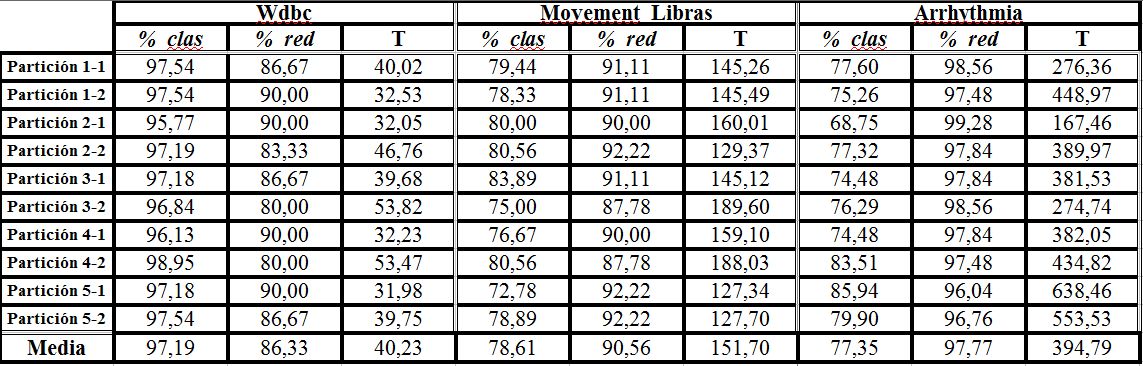
\includegraphics[scale=0.45]{Captura-SFS}

Búsqueda local:\\

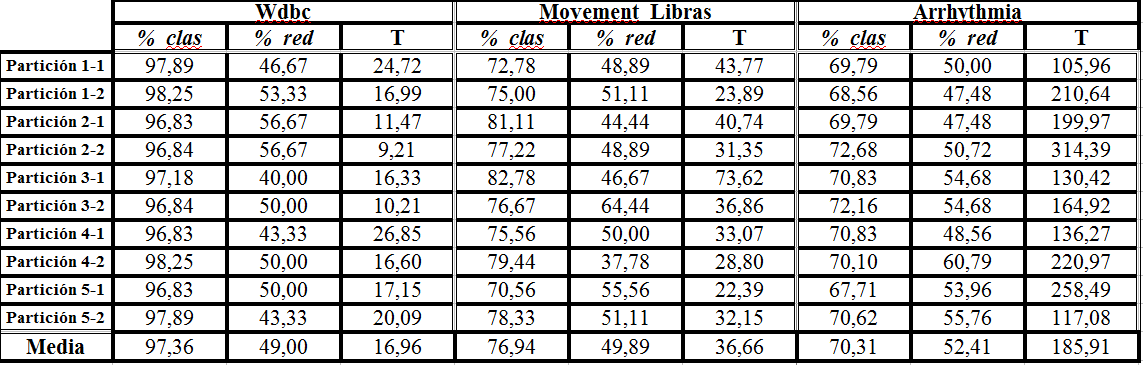
\includegraphics[scale=0.45]{Captura-BL}

Enfriamiento simulado:\\

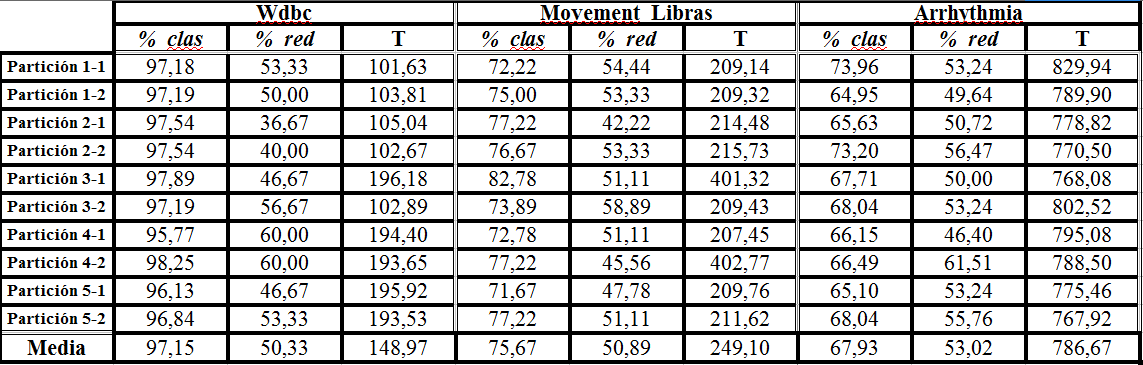
\includegraphics[scale=0.45]{Captura-SA}

Búsqueda tabú:\\

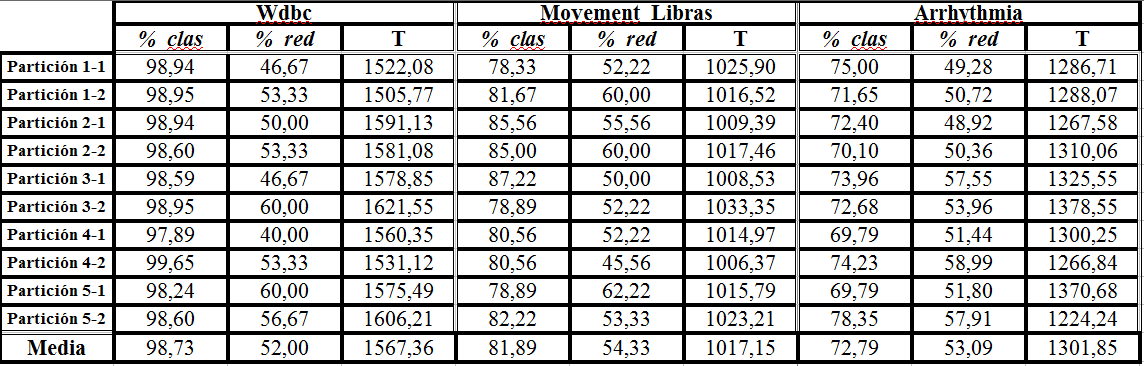
\includegraphics[scale=0.45]{Captura-TS}

Total:\\

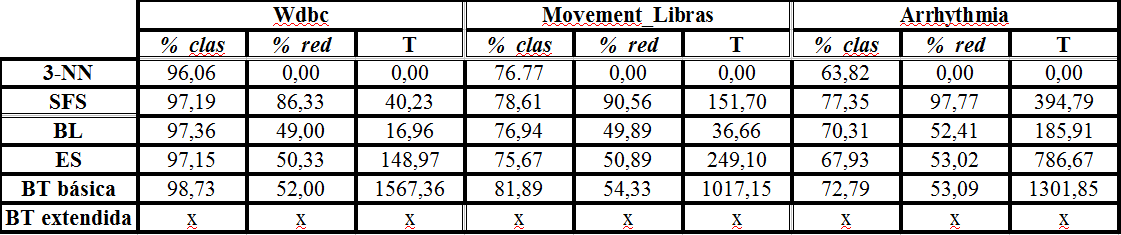
\includegraphics[scale=0.45]{Captura-fin}\\


Lo primero que podemos ver es que, con respecto al 3-NN conseguimos mejorar la clasificación en general, reduciendo el espacio de características a tener en cuenta. Esto es algo que podríamos esperar, pues muchos de esos datos podrían no tener importancia para el problema y ser fuente de ruido para clasificar. Por tanto, esto ya es de gran utilidad para el problema de clasificación.\\

En cuanto a las heurísticas, destacar primero la gran velocidad y el buen trabajo que hace la búsqueda local. Obtiene resultados buenos en muy poco tiempo comparado con los demás. Esto la hace atractiva para mejorar soluciones puntuales de manera muy rápida. Además, las soluciones de partida eran aleatorias, con posiciones de partida buenas --- obtenidas por otros procesos de búsqueda--- tiene que ser necesariamente aún más rápida. Esto lo seguiremos estudiando en las siguientes prácticas.\\

Por otro lado, el enfriamiento simulado no ha rendido como se esperaba. Sabiendo su funcionamiento, debería por lo menos igualar, si no mejorar, a la búsqueda local. Sin embargo, los resultados obtenidos son peores. Esto puede ser debido a que los parámetros no estén bien ajustados, probablemente por el cambio al máximo de 5000 iteraciones, pues los parámetros estaban ajustados para 15000.\\

La búsqueda Tabú gana en 2 de 3 bases de datos, y queda segunda en la otra. Advertir que esto se consigue en parte por ser la que más soluciones consigue explorar, esto lo podemos ver claramente en el tiempo empleado. Esto es así por ser la única de las búsquedas implementadas que siempre ejecuta el máximo de las iteraciones.\\

Destacar por último el tema de la reducción. Vemos como todas las heurísticas se quedan en torno al 50$\%$. Esto ya es una gran mejora, pero puede que haya momentos donde queramos quedarnos con menos datos aún. Para conseguir hacer esto, podríamos cambiar la función objetivo para que penalice el número de características que utiliza, pero con la versión de la función objetivo de la práctica, esto no se controla. \\

En resumen, viendo estos resultados, si necesitamos una búsqueda rápida, usaremos una búsqueda local. Para una búsqueda más profunda usando caminos, usaríamos la búsqueda tabú, a la que aún le podríamos hacer mejoras.\\
\newpage
\section{Referencias}
Aparte de la documentación de la asignatura, he usado las páginas de referencia del software usado para desarrollar las prácticas:
\begin{itemize}
\item Python:  \url{https://docs.python.org/3/}
\item Numpy y Scipy: \url{http://docs.scipy.org/doc/}
\item Scikit-learn: \url{http://scikit-learn.org/stable/documentation.html}
\end{itemize}
\end{document}